\documentclass[fleqn]{article}
\usepackage[nodisplayskipstretch]{setspace}
\usepackage{amsmath, nccmath, bm}
\usepackage{amssymb}
\usepackage{graphicx}
\usepackage{float}

\newcommand{\zerodisplayskip}{
	\setlength{\abovedisplayskip}{0pt}%
	\setlength{\belowdisplayskip}{0pt}%
	\setlength{\abovedisplayshortskip}{0pt}%
	\setlength{\belowdisplayshortskip}{0pt}%
	\setlength{\mathindent}{0pt}}
	
\title{Statistics and Probability}
\author{}
\date{}

\setlength{\parindent}{0pt}

\begin{document}
	\offinterlineskip
	\setlength{\lineskip}{12pt}
	\zerodisplayskip
	\maketitle
	
	A \underline{continuous random variable} $x$ can take on a continuum of values over some interval $(a,b)$ or over sets of intervals.
	
	The \underline{cummulative distribution function} (CDF) of a random variable $x$ is defined as
	
	\begin{equation*}
		F_X(a) \overset{\Delta}{=} \text{Probability}\{x \leq a\}
	\end{equation*}
	
	$F(a)$ is non-decreasing, $F(-\infty) = 0, F(\infty) = 1$
	
	The \underline{probability density function} (pdf) of a continuous random variable is defined as
	
	\begin{equation*}
		p(x) \overset{\Delta}{=} \frac{dF(x)}{dx}
	\end{equation*}
	
	$p(x) \geq 0$ and $\int_{-\infty}^{\infty}p(x)dx = 1$
	
	For the discrete random variable, we can use the probability mass function instead of the pdf.
	
	Let $X$ be a random variable with pdf $p_X(x)$. Let $Y = h(X)$. Then, the pdf of $Y$ is given by
	
	\begin{equation*}
		p_Y(y) = p_X(x) \cdot \left|\frac{dx}{dy}\right|
	\end{equation*}
	
	Expected value of $g(x) = E\{g(x)\} \overset{\Delta}{=}\int_{-\infty}^{\infty}g(x)p_X(x)dx$
	
	Mean $ = E\{x\} = \int_{-\infty}^{\infty}{xp_X(x)dx}$
	
	Variance $\sigma_X^2 = E\{x^2\} - E^2\{x\}$
	
	A continuous random variable can also be completely characterized by its \newline \underline{characteristic function}.
	
	\begin{equation*}
		Q_X(u) \overset{\Delta}{=} E\{e^{jux}\} = \int_{-\infty}^{\infty}{e^{jux}p_X(x)dx}
	\end{equation*}
	
	\begin{equation*}
		\therefore p_X(x) = \frac{1}{2\pi}\int_{-\infty}^{\infty}{Q_x(u)e^{-jux}du}
	\end{equation*}
	
	\begin{equation*}
		E\{x^n\} = (-j)^n\cdot\left.\frac{d^nQ_x(u)}{du^n}\right\vert_{u=0}
	\end{equation*}
	
	The \underline{joint CDF} of two random variables $X$ and $Y$ is
	
	$F_{X,Y}(a,b) = \text{Pr}\{X \leq a, Y \leq b\}$
	
	The \underline{joint pdf} is defined according to
	
	\begin{equation*}
		p_{X,Y}(x,y) \overset{\Delta}{=} \frac{\partial^2F_{X,Y}(x,y)}{\partial{x}\partial{y}}
	\end{equation*}
	
	The \underline{marginal pdfs} are given by
	
	\begin{equation*}
		p_X(x) = \int_{-\infty}^{\infty}p_{X,Y}(x,y)dy
	\end{equation*}
	
	\begin{equation*}
		p_Y(y) = \int_{-\infty}^{\infty}p_{X,Y}(x,y)dx
	\end{equation*}
	
	Two random variables are said to be \underline{statistically independent} if
	
	$p_{X,Y}(x,y) = p_X(x)p_Y(y)$
	
	Two random variabels are said to be \underline{uncorrelated} if
	
	$E\{XY\} = E\{X\}E\{Y\}$
	
	Note that statistical independence implies uncorrelatedness, but the converse is not generally true. (For Guassian random variables, statistical independence and uncorrelatedness are equivalent).
	
	$\text{COV}(X,Y) \overset{\Delta}{=} E\{(X-E[X])(Y-E[Y]) \} = E\{XY\} - E\{X\}E\{Y\}$
	
	The correlation coefficient $\rho$ betweeen $X$ and $Y$ is defined as
	
	\begin{equation*}
		\rho_{X,Y} \overset{\Delta}{=} \frac{\text{COV}(X,Y)}{\sigma_X\cdot\sigma_Y}
	\end{equation*}
	
	It can be shown that $-1 \leq \rho \leq 1$
	
	$\rho = +1$ implies a strong positive correlation between the two random variables.
	
	$\rho = 0$ implies no correlation
	
	$\rho = -1$ implies a strong negative correlation	
	
	For $N$ random variables $X_1, X_2,...,X_N$, we have statistical independence if
	
	\begin{equation*}
		p_{X_1, X_2,...,X_N}(x_1,x_2,...,x_N) = \prod_{j=1}^{N}p_{X_j}(x_j)
	\end{equation*}
	
	we can represent $N$ random variables compactly using a \underline{single} column vector
	
	\begin{equation*}
		\mathbf{X} = \begin{bmatrix} X_1, X_2,... ,X_N\end{bmatrix}^T
	\end{equation*}
	
	Then $p_\mathbf{X}(\mathbf{x})$ is a \underline{scalar} valued function of the vector $\mathbf{x}$ denoting the N-variate pdf of the $N$ random variables.
	
	The \underline{mean vector} of the random variable $\mathbf{X}$ is defined according to
	
	$\boldsymbol{\mu} = E\{\mathbf{x}\} \overset{\Delta}{=} \begin{bmatrix}E\{x_1\},E\{x_2\},...,E\{x_N\}\end{bmatrix}^T$
	
	Similarly, the \underline{covariance matrix} $\mathbf{\Sigma}$ is defined as
	
	$\mathbf{\Sigma} \overset{\Delta}{=} E\{(\mathbf{x} - \boldsymbol{\mu})(\mathbf{x} - \boldsymbol{\mu})^T\} = E\{\mathbf{X}\mathbf{X}^T\} - \boldsymbol{\mu}\boldsymbol{\mu}^T$
	
	Note that $\mathbf{\Sigma}$ is a $N \times N$ square, \underline{symmetric} matrix. In addition, it can be shown that $\mathbf{\Sigma}$ is a \underline{positive definite} matrix.
	
	When the $N$ random variables represented by $\mathbf{X}$ are statistically independent, $\mathbf{\Sigma}$ is a \underline{diagonal} matrix with the diagonal terms indicating the variances of the individual random variables.
	
	Let $Y_1, Y_2,...,Y_M$ be the random variables obtained from $X_1,X_2,...,X_N$ through the following \underline{linear} transformation.
	
	\begin{equation*}
		\begin{aligned}
			Y_1 &= a_{11}X_1 + a_{12}X_2 + \cdots + a_{1N}X_N \\
			Y_2 &= a_{21}X_1 + a_{22}X_2 + \cdots + a_{2N}X_N \\
			&\vdots \\
			Y_M &= a_{M1}X_1 + a_{M2}X_2 + \cdots + a_{MN}X_N
		\end{aligned}
	\end{equation*}
	
	Above linear relations can be expressed compactly using matrix notation as
	
	$\mathbf{Y} = \mathbf{AX}$
	
	where $\mathbf{X}$ is N-element column vector as defined before, $\mathbf{Y} = \begin{bmatrix}Y_1,Y_2,...,Y_M\end{bmatrix}^T$ is an M-element column vector and $\mathbf{A}$ is a $M \times N$ matrix with
	
	$A_{ij} = a_{ij}$, $1 \leq i \leq M$, $1 \leq j \leq N$
	
	as its i,jth element
	
	Then $\mathbf{\boldsymbol{\mu}_Y} = E\{\mathbf{Y}\} = \mathbf{A}E\{\mathbf{X}\} = \mathbf{A}\mathbf{\boldsymbol{\mu}_X}$
	
	$\mathbf{\Sigma_Y} = E\{(\mathbf{Y} - \mathbf{\boldsymbol{\mu}_Y})(\mathbf{Y} - \mathbf{\boldsymbol{\mu}_Y})^T\} = \mathbf{A}\mathbf{\Sigma_X}\mathbf{A}^T$
	
	This vector notation is very convenient when dealing with multiple random variables.
	
	Let $A$ and $B$ be two events with individual probabilities $P(A)$ and $P(B)$. Let $P(AB)$ denote the probability of the intersection of $A$ and $B$. Then the conditional probabilities are defined as
	
	\begin{equation*}
		P(A|B) \left[\text{This is read as "Probability of A given B"}\right]
	\end{equation*}
	
	\begin{equation*}
		= \frac{P(AB)}{P(B)}
	\end{equation*}
	
	Similarly
	
	\begin{equation*}
		P(B|A) = \frac{P(AB)}{P(A)}
	\end{equation*}
	
	If the events $A$ and $B$ are statistically independent, $P(A|B) = P(A)$ and $P(B|A) = P(B)$.
	
	This is known as \underline{Bayes theorem} and is of great significance in pattern recognition.
	
	\begin{figure}[H]
		\centerline{\fbox{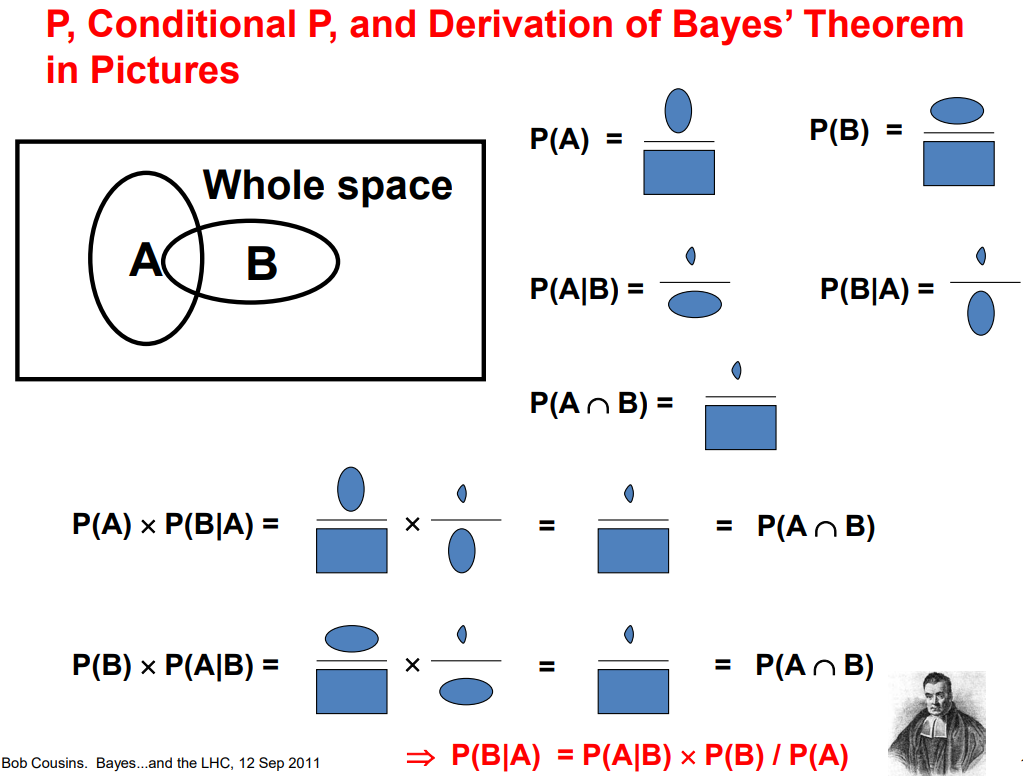
\includegraphics[width=0.9\textwidth]{bayes_rule.png}}}
		\caption{Bayes' Rule in Pictures}
		\label{bayes_rule}
	\end{figure}
	
	Let $X$ and $Y$ denote two continuous random variables. Then, the \newline \underline{conditional pdf} $p_{X|Y}(x|y)$ of $x$ given $y$ is
	
	\begin{equation*}
		p_{X|Y}(x|y) = \frac{p_{X,Y}(x,y)}{p_Y(y)}
	\end{equation*}
	
	Above important theorem can be stated in many different ways. We suppress the subscripts for convenience.
	
	\begin{equation*}
		p(x|y) = \frac{p(x,y)}{p(y)},\quad p(y|x) = \frac{p(x,y)}{p(x)}
	\end{equation*}
	
	\begin{equation*}
		\therefore p(x|y) = \frac{p(x,y)}{p(y)} = \frac{p(y|x)p(x)}{p(y)} = \frac{p(x)p(y|x)}{\int_{-\infty}^{\infty}{p(x)p(y|x)dx}}
	\end{equation*}
	
	If random variable $x$ is being determined by observing the random variable $y$, we use the notation:
	
	$p(x) = \text{"a priori" probability}$
	
	$p(y|x) = \text{conditional probability}$
	
	$p(x|y) = \text{"a posteriori" probability}$
	
	We provide a few examples of \underline{univariate} random variables below.
	
	\begin{enumerate}
		\item[(1)] \underline{Poisson:} The discrete random variable $n$ takes on integer values \newline $0,1,2,...,k,...$ till $\infty$
		
		\begin{equation*}
			\text{Pr}(n = k) = \frac{\lambda^k e^{-\lambda}}{k!},\quad\lambda > 0
		\end{equation*}
		
		$E\{n\} = \lambda$ and $\text{var}\{n\} = \lambda$
		
		\item[(2)] \underline{Binomial:} The discrete random variable $n$ takes on integer values \newline $0,1,2,...,N$.
		
		\begin{equation*}
			\text{Pr}(n = k) = \frac{N!}{k!(N-k)!}\theta^k(1 - \theta)^{(N - k)}, \quad k = 0,1,...,N
		\end{equation*}
		
		where $\theta$ is a parameter.
		
		$E\{n\} = N\theta$ and $\text{var}\{n\} = N\theta(1-\theta)$
		
		\item[(3)] \underline{Uniform:} The continuous random variable $x$ is governed by
		
		\begin{equation*}
			p(x) = \begin{cases}
				\frac{1}{(b-a)} & \text{for}\ a \leq x \leq b\\
				0 & \text{otherwise}
			\end{cases}
		\end{equation*}
		
		$E\{x\} = \left(\frac{a+b}{2}\right)$, the mid-point of the interval
		
		$var\{x\} = \frac{(b - a)^2}{12}$, one-twelfth of the square of the interval length.
		
		\item[(4)] \underline{Univariate Gaussian:} The continuous random variable $x$ has the following pdf.
		
		\begin{equation*}
			p(x) = \frac{1}{\sqrt{2\pi{\sigma_x}^2}}\text{exp}\left[-\frac{1}{2}\frac{(x-\mu_x)^2}{{\sigma_x}^2}\right]
		\end{equation*}
		
		$E\{x\} = \mu_x$ and $\text{var}\{x\} = {\sigma_x}^2$
		
		The univariate Guassian is \underline{completely} characterized by two parameters, namely, mean $\mu_x$ and variance ${\sigma_x}^2$
		
		For \underline{zero mean}, univariate Gaussian random variables, we can show the following.
		
		\begin{equation*}
			E\{x^p\} = \begin{cases}
				0 & \text{for odd}\ p\\
				\frac{p!}{\left(\frac{p}{2}\right)!2^{(p/2)}}\sigma^p & \text{for even}\ p
			\end{cases}
		\end{equation*}
			
		A univariate Gaussian pdf with mean $\mu$ and variance $\sigma^2$ is often denoted by $\mathcal{N}(\mu,\sigma^2)$
		
		The \underline{error function} $\text{erfc}(x)$ is defined as
		
		\begin{equation*}
			\text{erfc}(x) \overset{\Delta}{=} \frac{1}{\sqrt{2\pi}}\int_x^{\infty}{e^{-\frac{u^2}{2}}du}
		\end{equation*}
		
		$\text{erfc}(-\infty) = 1$, $\text{erfc}(0) = \frac{1}{2}$, $\text{erfc}(\infty) = 0$, $\text{erfc}(x) = 1 - \text{erfc}(x)$
		
		You can evaluate the error function on your calculator very accurately using the following algorithm.
		
		$\text{erfc}(x) = F(t)e^{-(x^2/2)}$
		
		$t = 1/(1 + 0.2316419x)$
		
		$F(t) = t\{0.127414796 + t\{-0.142248368 + t\{0.710706871$
		
		$+ t\{-0.726576013 + 0.530702714t\}\}\}\}$
		
		You may have to find $x$ such that
		
		$\beta = \text{erfc}(x),\quad 0 < \beta < \frac{1}{2}$
		
		Then $x$ can be obtained iteratively as below.
		
		Let $x_0$ be a guess for starting value.
		
		$t_0 = 1/(1 + 0.2316419x_0)$
		
		Find a new $x$ value from $x_0$ as
		
		\begin{equation*}
			x_1 = \left\{2\text{ln}\left[\frac{F(t_0)}{\beta}\right]\right\}^{1/2}
		\end{equation*}
		
		where $F(t)$ is the polynomial above.
		
		\item[(5)] \underline{Rayleigh:} The continuous random variable $x$ is governed by the following pdf.
		
		\begin{equation*}
			p(x) = \begin{cases}
				\frac{x}{b^2}e^{-\frac{x^2}{2b^2}} & \text{for}\ x \geq 0\\
				0 & \text{for} x < 0
			\end{cases}
		\end{equation*}
		
		\item[(6)] \underline{Gamma:} The continuous random variable $x$ is governed by the following pdf.
		
		\begin{equation*}
			p(x) = \begin{cases}
				\frac{1}{\Gamma(c)}x^{(c-1)}e^{-x} & \text{for}\ x \geq 0, c > 0\\
				0 & \text{for}\ x < 0
			\end{cases}
		\end{equation*}
		
		where the \underline{Gamma function} $\Gamma(c)$ is defined by
		
		\begin{equation*}
			\Gamma(c) \overset{\Delta}{=} \int_0^{\infty}x^{(c-1)}e^{-x}dx
		\end{equation*}
		
		Fortunately, we can use the recursion that
		
		$\Gamma(c+1) = c\Gamma(c)$ along with $\Gamma(1) = 1$, $\Gamma(\frac{1}{2}) = \sqrt{\pi}$, and $\Gamma(n) = (n-1)!$
		
		\item[(7)] \underline{Chi-squared:} The continuous random variable $x$ is governed by the following pdf.
		
		\begin{equation*}
			p(x) = \begin{cases}
				\frac{1}{2^{\beta/2}\Gamma\left(\frac{\beta}{2}\right)}x^{\left(\frac{\beta}{2} - 1\right)}e^{-\frac{x}{2}} & \text{for}\ x \geq 0\\
				0 & \text{for}\ x < 0
			\end{cases}
		\end{equation*}
		
		where $\beta$ is the \underline{number of degrees of freedom} associated with the chi-squared distribution
		
		The sum of squares of $N$ \underline{independent}, zero mean Gaussian variables with unit variance results in a chi-squared random variable with $N$ degrees of freedom
		
		Note also that if $x$ is a chi-squared random variable with $\beta$ degrees of freedom, then $(x/2)$ is a gamma random variable with the parameter \newline $c = (\beta/2)$.

	\end{enumerate}
\end{document}